%%%%%%%%%%%%%%%%%%%%%%%%%%%%%% Preamble
\documentclass[11pt]{article}
\setlength{\parskip}{\baselineskip}%
\setlength{\parindent}{0pt}%
\usepackage{amsmath,amssymb,amsthm,physics,graphicx,titling,hyperref}
\usepackage[margin=0.5in]{geometry}
\newcommand{\subtitle}[1]{%
  \posttitle{%
    \par\end{center}
    \begin{center}\large#1\end{center}
    \vskip0.5em}%
}

\usepackage{graphicx}
\begin{document}

%%%%%%%%%%%%%%%%%%%%%%%%%%%%%% Heading
	\title{Ph 21.2 - Introduction to Fourier Transforms}
	\author{Yovan Badal}
	\date{04/14/2018}
	\maketitle
	
%%%%%%%%%%%%%%%%%%%%%%%%%%%%%% Body
\section{Properties and Consistency of the Fourier Series}
\begin{enumerate}
	\item We prove the consistency of eqns (2) and (3) as respective definitions of the inverse Fourier series and Fourier series.
	\begin{align}
		\sum_{k=-\infty}^{\infty} \tilde h_k e^{-2\pi i f_k x} =& \sum_{k=-\infty}^{\infty} e^{-2\pi i f_k x} \frac{1}{L} \int_0^L h(x')  e^{2\pi i f_k x'} \dd{x'} \\
		=& \int_0^L \sum_{k=-\infty}^{\infty} \frac{1}{L} h(x') e^{-2\pi i \frac{k}{L} (x'-x)} \dd{x'} \\
		=& \int_{-\infty}^{-\infty} \int_{-\infty}^{\infty} \frac{1}{L} h(x') e^{-2\pi i \frac{k}{L} (x'-x)} \dd{k} \dd{x'} \\
		=& \int_{-\infty}^{-\infty} h(x') \int_{-\infty}^{\infty} e^{-2\pi i k' (x'-x)} \dd{k'} \dd{x'} \\
		=& \int_{-\infty}^{-\infty} h(x') \delta(x'-x) \dd{x'} \\
		=& h(x)
	\end{align}
	where in line (3) we change the bounds of our $x$-integral by setting for convenience our function $h(x)$ to be $0$ outside of $x \in [0,L)$ and we use the fact that the signal we are concerned with is periodic to replace the infinite sum over $k$ with an indefinite k-integral. This is because the Fourier \textit{transform}, given by $H(k)=\int_{-\infty}^{\infty} h(x) e^{2 \pi i k x}\dd{x}$ (an extension of sorts of the Fourier series used to analyze aperiodic signals) of a periodic signal $h(x)$ consists of a sum of delta-distributions, which reduces the integral $H(k)$ to an infinte sum of complex exponetials over integer $k$. In line (4), we use a simple change of variables, in line (5) we use the Fourier transform of the dirac-delta distribution, and in line (6) we use the fundamental property of the dirac-delta distribution.
	
	\newpage
	\item We work out a special case of the completeness of complex exponentials.
	\begin{align}
		A\sin (2 \pi x/L + \varphi) &= \frac{i A}{2}(e^{-i(2 \pi x/L + \varphi)} - e^{i(2 \pi x/L + \varphi)}) \\
		&= \frac{i A}{2} \big(e^{-i \varphi} e^{-2 \pi i x/L} - e^{i \varphi} e^{2 \pi i x/L}\big) \\
		&= \bigg(\frac{i A}{2} e^{-i \varphi}\bigg) e^{-2 \pi i x/L} - \bigg(\frac{i A}{2} e^{i \varphi}\bigg) e^{2 \pi i x/L}
	\end{align}
	where in line (7) we have used DeMoivre's theorem. This proves the claim.
	
	\item We demonstrate a property of the Fourier coefficients for real $h(x)$.
	\begin{align}
		\tilde h_{-k} &= \frac{1}{L} \int_0^L h(x) e^{2 \pi i f_{-k} x} \dd{x} \\
		=& \frac{1}{L} \int_0^L h(x) e^{-2 \pi i f_{k} x} \dd{x} \\
		=& \frac{1}{L} \int_0^L h(x) \big[ e^{2 \pi i f_{k} x} \big]^{*} \dd{x} \\
		=& \bigg[ \frac{1}{L} \int_0^L h(x) e^{2 \pi i f_{k} x} \dd{x} \bigg]^{*} \\
		=& \tilde h_k^*
	\end{align}
	where in line (11) we have used the definition $f_k = \frac{k}{L}$, in line (12) we have used an obvious property of the complex exponential (which can easily be seen using DeMoivre's theorem) and in line (13) we have used the fact that $h(x)$ and our integration variable $x$ are real.
	
	\item We prove a version of the convolution theorem for Fourier series. Let $H(x) = h^{(1)}(x) h^{(2)}(x)$. Then we can write the Fourier series for $h^{(1)}(x)$ and $h^{(2)}(x)$:
	\begin{align}
	h^{(1)}(x) =& \sum_{k=-\infty}^{\infty} \tilde h_k^{(1)} e^{-2 \pi i f_k x} \\
	h^{(2)}(x) =& \sum_{k=-\infty}^{\infty} \tilde h_k^{(2)} e^{-2 \pi i f_k x}
	\end{align}
	such that we can write $H(x)$ as:
	\begin{align}
	H(x) =& h^{(1)}(x) h^{(2)}(x) \\
	=& \bigg( \sum_{k=-\infty}^{\infty} \tilde h_k^{(1)} e^{-2 \pi i f_k x} \bigg) \bigg( \sum_{k=-\infty}^{\infty} \tilde h_k^{(2)} e^{-2 \pi i f_k x} \bigg) \\
	=& \sum_{k=-\infty}^{-\infty} \bigg( \sum_{k'=-\infty}^{\infty} \tilde h_{k-k'}^{(1)} \tilde h_{k'}^{(2)} \bigg) e^{-2 \pi i f_k x}
	\end{align}
	and we can then find the Fourier coefficents $H_k$ of $H(x)$ as follows:
	\begin{align}
	H_k =& \frac{1}{L} \int_0^L H(x) e^{2 \pi i f_k x} \dd{x} \\
	=& \frac{1}{L} \int_0^L \sum_{l=-\infty}^{\infty} \bigg( \sum_{k'=-\infty}^{\infty} \tilde h_{l-k'}^{(1)} \tilde h_{k'}^{(2)} \bigg) e^{-2 \pi i f_l x} e^{2 \pi i f_k x} \dd{x} \\
	=& \frac{1}{L} \int_0^L \sum_{l=-\infty}^{\infty} \bigg( \sum_{k'=-\infty}^{\infty} \tilde h_{l-k'}^{(1)} \tilde h_{k'}^{(2)} \bigg) e^{2 \pi i (f_k - f_l) x} \dd{x} \\
	=& \frac{1}{L} \sum_{l=-\infty}^{\infty} \bigg( \sum_{k'=-\infty}^{\infty} \tilde h_{l-k'}^{(1)} \tilde h_{k'}^{(2)} \bigg) \int_0^L e^{2 \pi i (f_k - f_l) x} \dd{x} \\
	\end{align}
	Now, observe that $\int_0^L e^{2 \pi i (f_k - f_l) x} \dd{x} = \big\{_{0 \ \text{else}}^{L \ k=l}$ since we are integrating over an integer number of periods of the complex exponential. Therefore:
	\begin{align}
	H_k =& \sum_{k'=-\infty}^{\infty} \tilde h_{k-k'}^{(1)} \tilde h_{k'}^{(2)}
	\end{align}
	\textit{Graphical interpretation of the convolution product:} If we imagine a graphical interpretation of the \textit{spectrum} of a periodic function $h(x) = \sum_{k=-\infty}^{\infty} \tilde h_k e^{-2 \pi i f_k x}$ (the representation of the function $h(x)$ in $k$-space given by its Fourier series) as a graph of impulses ($\delta$-distributions) at $k$ scaled by $h_k$, we can represent the convolution product $H(x)$ as defined above as follows: we consider the spectrum of $h^{(1)}(x)$ (WLOG since convolution is clearly commutative by the above) as described above. We then consider the spectrum of $h^{(2)}(x)$, reflect it with respect to $k$ (i.e. $k \mapsto -k$) and offset it by $k'$ (i.e. $k \mapsto k + k'$). We then superpose the two spectra, multiply the scaling factors of the impulses superposed at every $k$, and sum the products over $k$ to obtain $H_{k'}$ (Note: in the limit of continuous spectra given by the Fourier transform, this sum becomes an integral represented in the above by the area under the product of the superposed spectra described above).
	
	\textit{Example (smooth $h_k^{(1)}$ centered at $k=0$, $h_k^{(2)} = \delta_{k, 50}$):}

\begin{figure}[!htbp]
  \begin{minipage}[b]{0.5\textwidth}
    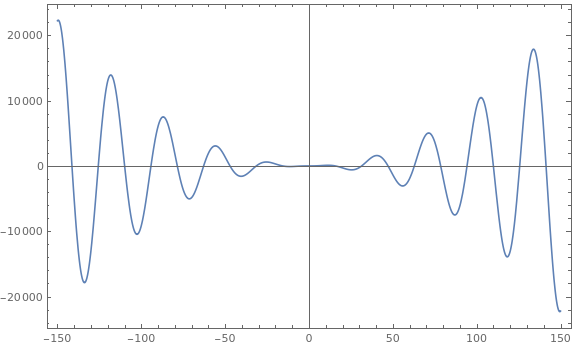
\includegraphics[width=\textwidth]{smooth_conv.png}
    \caption{$\tilde h_k^{(1)}$}
  \end{minipage}
  \hfill
  \begin{minipage}[b]{0.5\textwidth}
    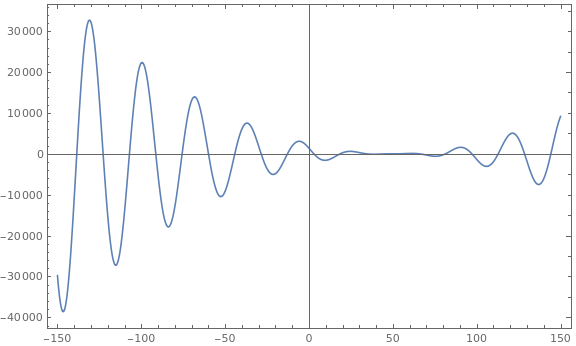
\includegraphics[width=\textwidth]{smooth_conv_shift.png}
    \caption{$\tilde H_k$}
  \end{minipage}
\end{figure}
	We observe that the convolution is simply the spectrum $h_k^{(1)}$ shifted forwards by 50 (i.e., $\tilde H_k$ = $h_{k-50}^{(1)}$).
\newpage

	\item We test the numpy fft function by first working out the expected spectrum for a function (in our case a cosine then a Gaussian) and observing whether the fft output matches our expected spectrum. Then we use the inverse fft (ifft in numpy) to recover our function and verify that we actually recover our input.
	
	\textbf{Cosine function:} For a function of the form $C + A \cos (ft+\varphi)$, we expect the spectrum to be two delta peaks, one at $f=0$ corresponding to the offset $C$, and the other at frequency $f$. When displaying the spectrum, we will be plotting the absolute values of the Fourier coefficients $h_k$, and therefore our spectrum plot will disregard any phase shift $\varphi$ since phase shift will change the complex value of $h_k$ but not it's absolute value (i.e. it will rotate the phasor corresponding the $h_k$ in the complex plane.
	
\begin{figure}[htp]
\centering
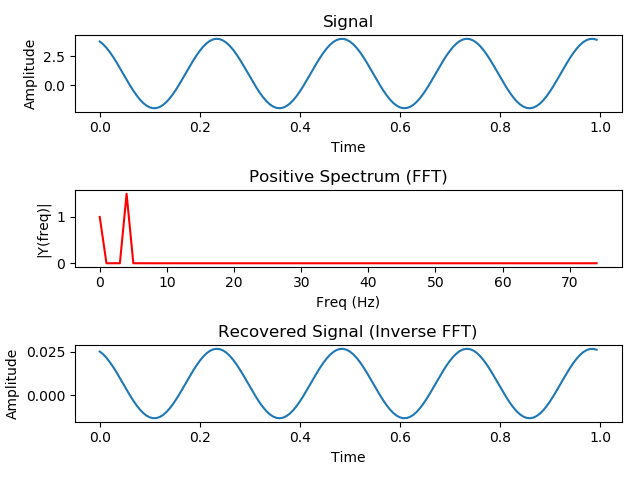
\includegraphics[scale=1.00]{cosine_signal.png}
\caption{Plot of the signal $h(t)=1 + 3 \cos (4t+0.1)$, its spectrum, and the signal recovered from the spectrum using the inverse FFT. All the expected features mentioned above are observed, indicating a successful test of numpy's FFT. The amplitudes of the peaks in the spectrum correspond to the absolute values of $h_k$.}
\label{cos_signal}
\end{figure}
	\newpage
	\textbf{Gaussian function:} First, we find the Fourier series of the Gaussian function $h(t) = e^{-B(t-\frac{L}{2})^2}$:
	\begin{align}
	\tilde h_k =& \frac{1}{L} \int_0^L h(t) e^{2 \pi i f_{k} t} \dd{t} \\
	=& \frac{1}{L} \int_0^L A e^{-B(t-\frac{L}{2})^2} e^{2 \pi i f_{k} t} \dd{t} \\
	=& \frac{1}{L} \int_{-\frac{L}{2}}^{\frac{L}{2}} A e^{-Bt^2} e^{2 \pi i f_k (t + \frac{L}{2})} \dd{t} \\
	=& \frac{1}{L} \int_{-\frac{L}{2}}^{\frac{L}{2}} A e^{-Bt^2} e^{2 \pi i f_k t} e^{\pi i k}\dd{t} \\
	=& \frac{e^{\pi i k}}{L} \int_{-\frac{L}{2}}^{\frac{L}{2}} A e^{-Bt^2} e^{2 \pi i f_k t} \dd{t} \\
	=& \frac{e^{\pi i k}}{L} \int_{-\frac{L}{2}}^{\frac{L}{2}} A e^{-Bt^2} [\cos (2 \pi f_k t) + i \sin (2 \pi f_k t)] \dd{t} \\
	=& \frac{A e^{\pi i k}}{L} \bigg[ \int_{-\frac{L}{2}}^{\frac{L}{2}} e^{-Bt^2} \cos (2 \pi f_k t) \dd{t} + i \int_{-\frac{L}{2}}^{\frac{L}{2}} e^{-Bt^2} \sin (2 \pi f_k t)] \dd{t} \bigg] \\
	=& \frac{A e^{\pi i k}}{L} \int_{-\frac{L}{2}}^{\frac{L}{2}} e^{-Bt^2} \cos (2 \pi f_k t) \dd{t} \\
	=& \frac{A e^{\pi i k}}{L} \int_{-\infty}^{\infty} e^{-Bt^2} \cos (2 \pi f_k t) \dd{t} \\
	=& \frac{A e^{\pi i k}}{L} \sqrt{\frac{\pi}{B}} e^{\frac{-\pi^2 f_k^2}{B}} \\
	=& \bigg\{^{\sqrt{\frac{\pi A^2}{B L^2}} e^{\frac{-\pi^2 k^2}{B L^2}} \ \text{$k$ is even}}_{-\sqrt{\frac{\pi A^2}{B L^2}} e^{\frac{-\pi^2 k^2}{B L^2}} \ \text{$k$ is odd}}
	\end{align}
	where in line (28) we have used the change of variables $t \mapsto t+\frac{L}{2}$, in line (31) we used DeMoivre's theorem, in line (33) we used the fact that the second term in line (32) has an odd integrand (the exponential factor is clearly even, and sin is odd so their product is odd) and therefore integrates to zero over symmetric bounds, in line (34) we have changed the bounds by taking the approximation that for $B>>L$ ('B large enough' as mentioned in the question) the Gaussian goes to zero near the bounds and outside, and finally in line (35) we look up the integral (found on Wolfram Mathworld).
	
	We can then expect that the spectrum of the Gaussian is even and oscillates between positive and negative values depending on the parity of $k$ as described above, with amplitude decaying as a scaled Gaussian centered at 0 with increasing absolute value of $k$
	\begin{figure}[htp]
	\centering
	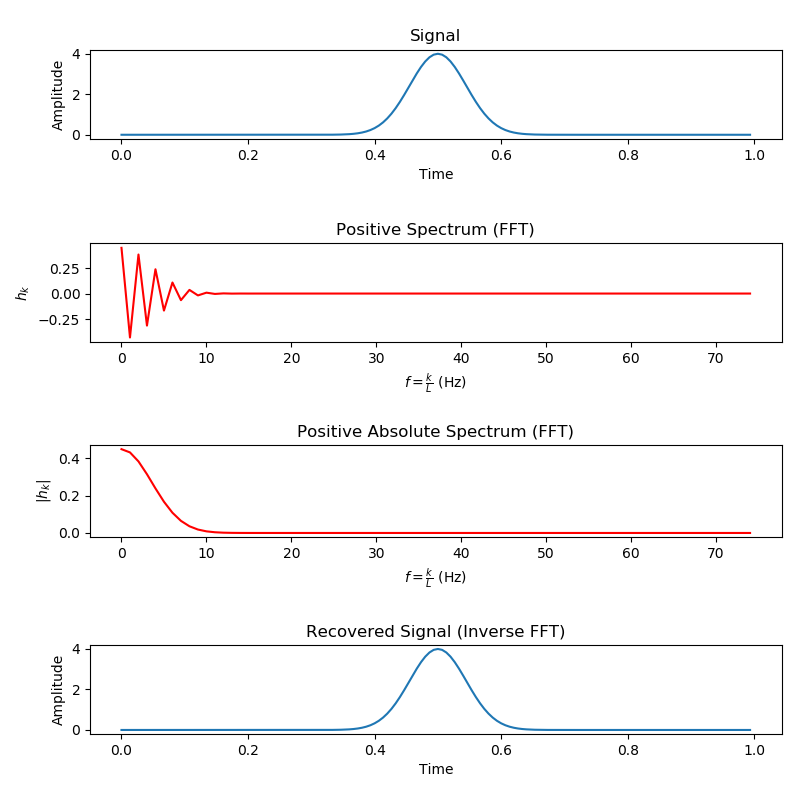
\includegraphics[scale=0.90]{gaussian_signal.png}
	\caption{This is for a Gaussian with $A=4$ and $B=250$. As expected, the spectrum oscillates between positive and negative values with decaying amplitude with increasing absolute value of $k$, and the absolute value spectrum is simply a scaled Gaussian. The signal is recovered by the Inverse FFT as desired. From our work above, we calculate an expected value for $h_0$ of 0.44840, and this is almost exactly the value we observe on our spectrum by printing the $0^{th}$ element of the FFT array. This indicates another successful test of numpy's FFT.}
	\label{gaussian_signal}
	\end{figure}. Furthermore, the absolute value spectrum of a Gaussian should be a scaled Gaussian centered at 0.
\end{enumerate}

	\newpage
\section{Analysis of Arecibo Data}
\begin{enumerate}
\item The Fourier spectrum for Arecibo Data is shown below:
\begin{figure}[!hbtp]
\centering
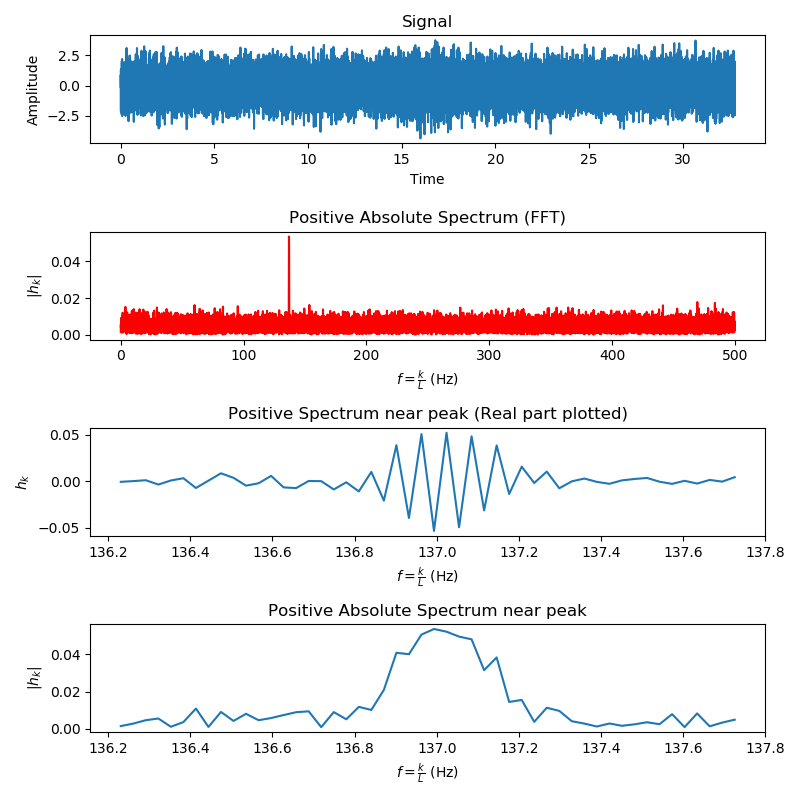
\includegraphics[scale=0.90]{arecibo_plot.png}
\caption{Plots of Arecibo data in time-domain and frequency-domain (the latter obtained using FFT) showing a peak and global maximum at 1420.000137 MHz (recall that the frequencies in the spectrum above are shifted backwards by 1420 MHz). Observe that we do not obtain a sharp peak in the absolute-value spectrum at the signal frequency as we would have for a sinusoidal signal; we obtain a rather rounded peak around the maximum, reminescent of a shifted Gaussian. This is also supported by the oscillation around the peak in the (non-absolute) spectrum.}
\label{arecibo_1}
\end{figure}
\newpage

	\item As mentioned above, the shape of the Fourier spectrum peak is indicative of a shifted Gaussian. We therefore attempt a Gaussian+Constant fit using CurveFit (Mathematica package provided for sophomore labs) and obtain the following:
	\begin{figure}[htp]
	\centering
	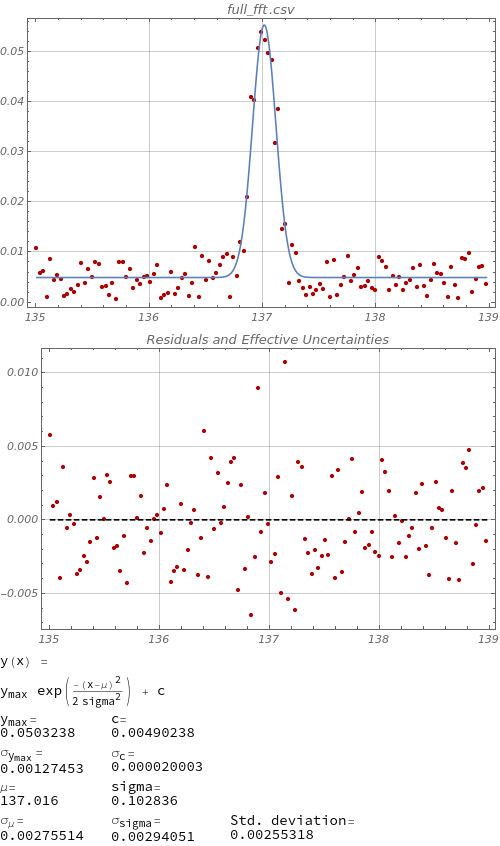
\includegraphics[scale=0.58]{curvefit_arecibo_fft_1.png}
	\caption{Plot of fit and fit parameters for a Gaussian+Linear fit on our absolute value Fourier spectrum obtained using Curvefit. Peak is found as expected at 1420.000137 MHz, and we observe a qualitatively reasonably good fit (we cannot do a $\tilde \chi^2$ or other goodness-of-fit test because we are not given estimates for the uncertainties on our data).}
	\label{curvefit_fft_1}
	\end{figure}
	
	\newpage
	Now, we observe that a shifted Gaussian spectrum can be expressed as the convolution product of a Gaussian spectrum and a delta-peak spectrum. From our work in part I, we can therefore expect the signal to be a Gaussian multiplied by a sinusoidal signal. By a slight modification of our proof for the Fourier spectrum of a Gaussian, we can conclude that knowing $t_0$, the time about which the Gaussian factor is centered, is not important to finding the time constant $\Delta t$ of the envelope: to account for general centerings other than $t_0 = \frac{L}{2}$, we simply have to modify the complex exponential factor in our result, and obtain:
	\[
	\tilde h_k = e^{2 \pi i f_k t_0}\sqrt{\frac{\pi A^2}{B L^2}} e^{\frac{-\pi^2 f_k^2}{B}}
	\]
	which still has absolute value
	\[
	|\tilde h_k| = \sqrt{\frac{\pi A^2}{B L^2}} e^{\frac{-\pi^2 f_k^2}{B}}
	\]
	as before. Therefore, we can use our fit parameters for the absolute-value spectrum of our data to estimate $\Delta t$ by equating the variances as follows:
	\begin{align}
		\frac{\pi^2}{B} =& \frac{1}{2 \sigma^2} \\
		\pi^2 (\Delta t)^2 =& \frac{1}{2 \sigma^2} \\
		\Delta t =& \frac{1}{\sqrt{2} \pi \sigma} \\
		=& 2189 \ ms
	\end{align}
	We visually verify our estimate by superposing a plot of the signal's FFT obtained above with the FFT of a Gaussian envelope with $\Delta t = 2.189 \ s$.
	\begin{figure}[htp]
	\centering
	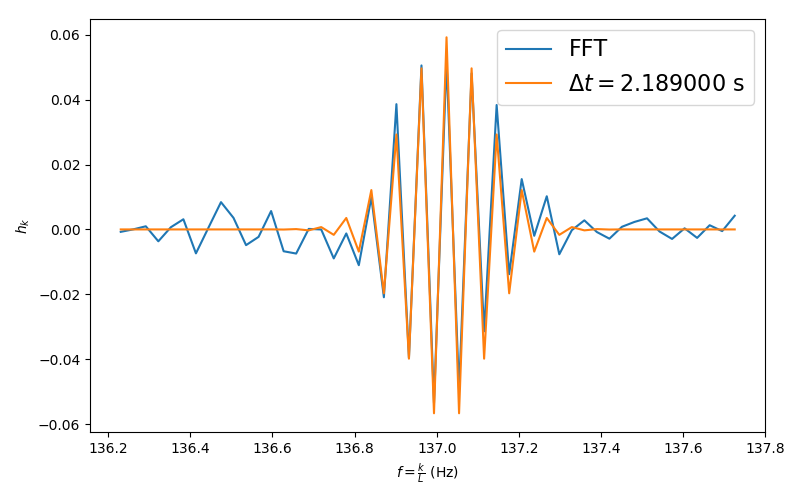
\includegraphics[scale=0.70]{dt_compare.png}
	\caption{Superimposed plots of the real part of the Fourier spectrum of our signal, and of the spectrum of a Gaussian envelope with $\Delta t = 2.189 \ s$. Note that the FFT of the Gaussian has been shifted to account for the convolution with a delta peak at the signal frequency such that our plots coincide as observed. Furthermore, we have roughly scaled the FFT of the Gaussian such that it is easier to make a visual comparison using the superposition.}
	\label{comp_1}
	\end{figure}
	\newpage
	
	We observe that our predicted envelope matches quite well with the width of the FFT of our signal, indicating that our guess for $\Delta t = 2.189 \ s$ was resonably accurate. For comparison, we present a similar plot with a range of $\Delta t$'s.
	\begin{figure}[htp]
\centering
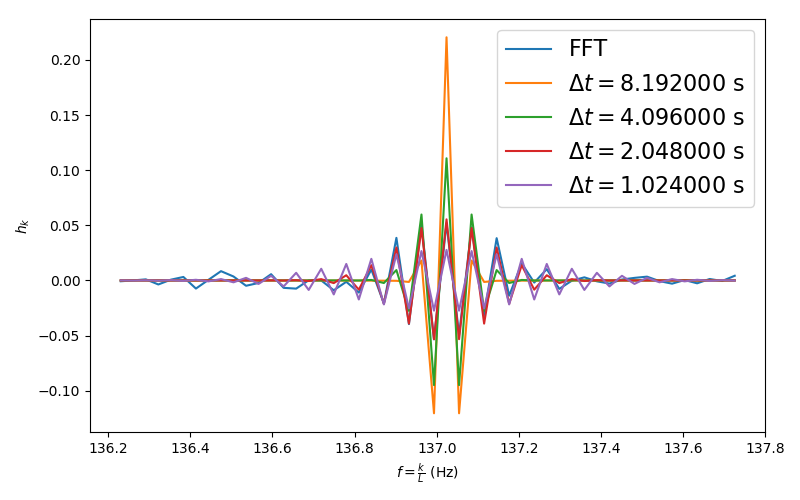
\includegraphics[scale=0.70]{dt_compare_others.png}
\caption{Superimposed plots of the real part of the Fourier spectrum of our signal, and of the spectrum of appropriately shifted and scaled Gaussian envelopes with $\Delta t$'s as labelled. We can observe that the best match between the envelopes and the FFT of our signal occurs for $\Delta t = 2.05 \ s$, i.e. when $\Delta t$ is the closest to our estimate. However, it is still apparent by comparing with the plot above that our estimate produces the best match between the predicted envelope and the FFT of our signal.}
\label{comp_2}
\end{figure}
\end{enumerate}
\newpage

\section{Unequally Sampled Data and the Lomb-Scargle Algorithm}

\end{document}